\section{Optimization and Lagrange Multipliers}

\subsection{Optimization}

\begin{definition}{Local Maximum and Minimum}{local_max_min}
For a function $f(x, y)$ and a point $(a, b)$ in its domain, we say that $(a, b)$ is a 
\begin{itemize}
    \item \textbf{local maximum} if $f(a, b) \geq f(x, y),\ \forall (x, y)$ in a neighborhood of $(a, b)$.
    \item \textbf{local minimum} if $f(a, b) \leq f(x, y),\ \forall (x, y)$ in a neighborhood of $(a, b)$.
\end{itemize}
\end{definition}

\begin{figure}[htbp]
\centering
\begin{minipage}{0.48\textwidth}
\centering
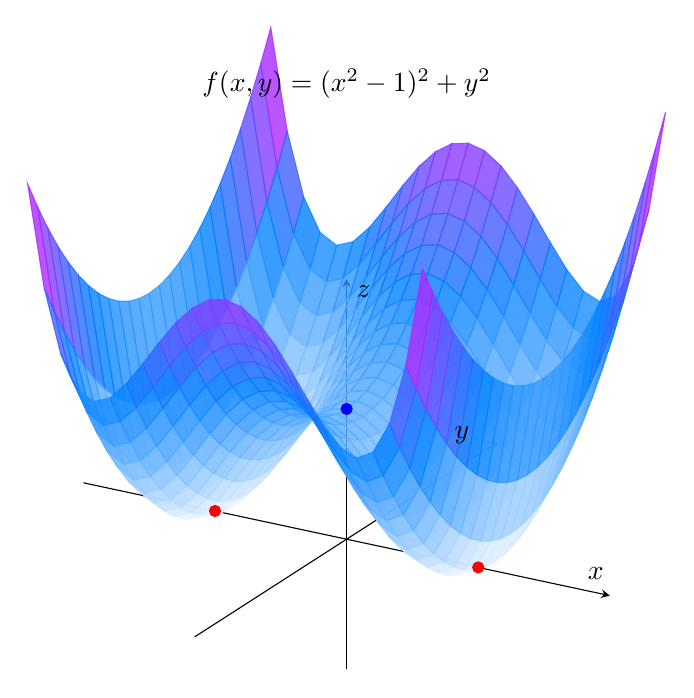
\begin{tikzpicture}
\begin{axis}[
    view={30}{30},
    axis lines=center,
    xlabel={$x$},
    ylabel={$y$},
    zlabel={$z$},
    xmin=-2, xmax=2,
    ymin=-1.5, ymax=1.5,
    zmin=-1, zmax=2,
    ticks=none,
    clip=false,
    width=\textwidth,
    title={$f(x,y) = (x^2-1)^2 + y^2$}
]
    % Quartic double well potential surface
    \addplot3[
        surf,
        domain=-1.5:1.5,
        domain y=-1.2:1.2,
        samples=25,
        colormap/cool,
        opacity=0.8,
        faceted color=none
    ]
    ({x}, {y}, {(x^2 - 1)^2 + y^2});

    % Highlight Minima at (-1,0) and (1,0)
    \addplot3[mark=*, mark size=2pt, color=red] coordinates {(-1, 0, 0)};
    \addplot3[mark=*, mark size=2pt, color=red] coordinates {(1, 0, 0)};
    % Highlight Saddle/Max at (0,0)
    \addplot3[mark=*, mark size=2pt, color=blue] coordinates {(0, 0, 1)};
\end{axis}
\end{tikzpicture}
\end{minipage}%
\end{figure}

\begin{definition}{Critical Point}{critical_point}
We call a point $P(a, b)$ a \textbf{critical point} of $f$ if
\[
\nabla f(P) = \vv{0}
\]
\end{definition}

\begin{theorem}{Critical Points and Local Extrema}{critical_points_local_extrema}
If $P(a, b)$ is a local extremum of $f$, then $P$ is a critical point of $f$.
\end{theorem}

For single variable functions, we can use the second derivative test to determine the nature of a point on the function.
For $f(x)$, if $f'(a) = 0$, then:
\begin{itemize}
    \item If $f''(a) > 0$, then $f$ has a local minimum at $x = a$.
    \item If $f''(a) < 0$, then $f$ has a local maximum at $x = a$.
    \item If $f''(a) = 0$, the test is inconclusive.
\end{itemize}